% Options for packages loaded elsewhere
\PassOptionsToPackage{unicode}{hyperref}
\PassOptionsToPackage{hyphens}{url}
%
\documentclass[
  11pt,
  letter]{article}
\usepackage{amsmath,amssymb}
\usepackage{lmodern}
\usepackage{iftex}
\ifPDFTeX
  \usepackage[T1]{fontenc}
  \usepackage[utf8]{inputenc}
  \usepackage{textcomp} % provide euro and other symbols
\else % if luatex or xetex
  \usepackage{unicode-math}
  \defaultfontfeatures{Scale=MatchLowercase}
  \defaultfontfeatures[\rmfamily]{Ligatures=TeX,Scale=1}
  \setmainfont[]{NanumMyeongjo}
\fi
% Use upquote if available, for straight quotes in verbatim environments
\IfFileExists{upquote.sty}{\usepackage{upquote}}{}
\IfFileExists{microtype.sty}{% use microtype if available
  \usepackage[]{microtype}
  \UseMicrotypeSet[protrusion]{basicmath} % disable protrusion for tt fonts
}{}
\makeatletter
\@ifundefined{KOMAClassName}{% if non-KOMA class
  \IfFileExists{parskip.sty}{%
    \usepackage{parskip}
  }{% else
    \setlength{\parindent}{0pt}
    \setlength{\parskip}{6pt plus 2pt minus 1pt}}
}{% if KOMA class
  \KOMAoptions{parskip=half}}
\makeatother
\usepackage{xcolor}
\usepackage[margin=1in]{geometry}
\usepackage{graphicx}
\makeatletter
\def\maxwidth{\ifdim\Gin@nat@width>\linewidth\linewidth\else\Gin@nat@width\fi}
\def\maxheight{\ifdim\Gin@nat@height>\textheight\textheight\else\Gin@nat@height\fi}
\makeatother
% Scale images if necessary, so that they will not overflow the page
% margins by default, and it is still possible to overwrite the defaults
% using explicit options in \includegraphics[width, height, ...]{}
\setkeys{Gin}{width=\maxwidth,height=\maxheight,keepaspectratio}
% Set default figure placement to htbp
\makeatletter
\def\fps@figure{htbp}
\makeatother
\setlength{\emergencystretch}{3em} % prevent overfull lines
\providecommand{\tightlist}{%
  \setlength{\itemsep}{0pt}\setlength{\parskip}{0pt}}
\setcounter{secnumdepth}{-\maxdimen} % remove section numbering
\usepackage{kotex}
\usepackage{setspace}
\doublespacing
\usepackage{float}
\floatplacement{figure}{htbp}
\usepackage{longtable}
\usepackage[hang]{footmisc}
\setlength{\footnotemargin}{2mm}
\ifLuaTeX
  \usepackage{selnolig}  % disable illegal ligatures
\fi
\IfFileExists{bookmark.sty}{\usepackage{bookmark}}{\usepackage{hyperref}}
\IfFileExists{xurl.sty}{\usepackage{xurl}}{} % add URL line breaks if available
\urlstyle{same} % disable monospaced font for URLs
\hypersetup{
  hidelinks,
  pdfcreator={LaTeX via pandoc}}

\title{\Large \bf 민주화 이후 한국 국회의원 재보궐 선거 데이터 코드북}
\usepackage{etoolbox}
\makeatletter
\providecommand{\subtitle}[1]{% add subtitle to \maketitle
  \apptocmd{\@title}{\par {\large #1 \par}}{}{}
}
\makeatother
\subtitle{\large Coodbook for General Re/By-Election of South Korea}
\author{Sanghoon Park\footnote{Department of Political Science,
  University of South Carolina, Columbia, 29208, 817 Henderson Street,
  Columbia, S.C., United States; \url{pherephobia@gmail.com}}}
\date{2022-8-23}

\begin{document}
\maketitle
\begin{abstract}
\noindent 1989년 4월 14일부터 2022년 6월 1일까지의 재보궐 146개 선거가
분석대상이며, 이에 대한 자료는 중앙선거관리위원회의 홈페이지의
선거통계시스템(\url{http://info.nec.go.kr)과} 중앙선거관리위원회가
편찬한 '대한민국선거사'를 통해 획득하였다.
\end{abstract}

{
\setcounter{tocdepth}{3}
\tableofcontents
}
\clearpage
\newpage

\hypertarget{data-descriptions}{%
\section{Data Descriptions}\label{data-descriptions}}

\hypertarget{uxc7acuxbcf4uxad90-uxc120uxac70-uxbcc0uxc218}{%
\subsection{재보궐 선거
변수}\label{uxc7acuxbcf4uxad90-uxc120uxac70-uxbcc0uxc218}}

\begin{description}
\item[\textbf{ELEC\_DATE}]
선거일(DATE), 재보궐선거가 실시된 연-월-일 (1989년 민주화 이후의
시점(1989-04-14)부터 현재(2022-8-23)까지 최신화).
\end{description}

\begin{figure}
\centering
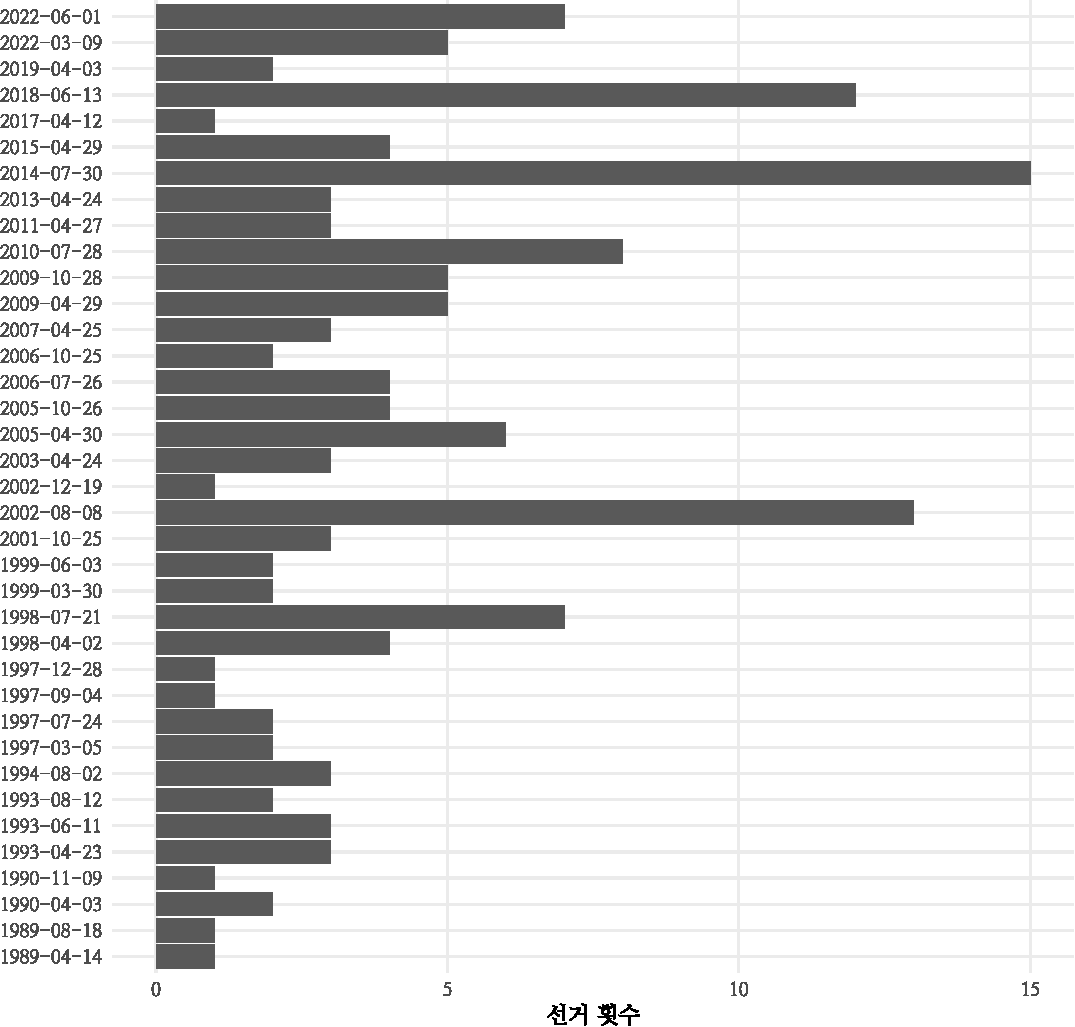
\includegraphics{Codebook_national_files/figure-latex/unnamed-chunk-1-1.pdf}
\caption{재보궐 선거의 추이}
\end{figure}

\begin{description}
\item[ELEC\_TYPE]
선거유형(CHR), 선출유형에 따른 분류 (현재는 국회의원만 코딩).
\item[CITY]
시도(CHR), 시도 구분.
\item[DISTRICT]
선거구(CHR), 선거구명.
\item[ELEC\_POP]
선거인수(NUM), 총 유권자 수.
\item[ELEC\_VOTER]
투표수(NUM), 총 투표인 수.
\item[ELEC\_RESIGN]
기권자수(NUM) 총 유권자 수 - 총 투표인 수.
\item[ELEC\_TURNOUT]
투표율(NUM) 총 투표인 수 / 총 유권자 수 * 100.
\end{description}

\begin{figure}
\centering
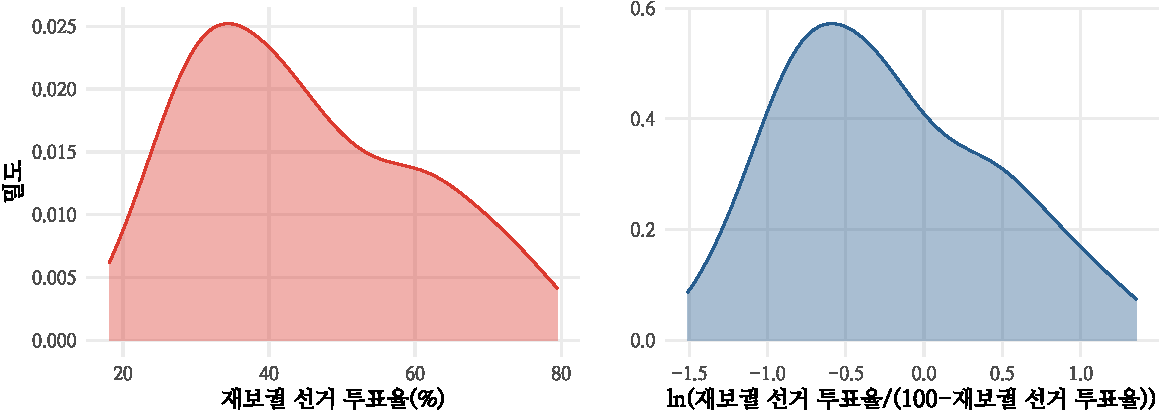
\includegraphics{Codebook_national_files/figure-latex/unnamed-chunk-2-1.pdf}
\caption{재보궐 선거 투표율 변수의 분포}
\end{figure}

\begin{description}
\item[ELEC\_REASON]
사유(FCT) 재보궐 시행 사유.
\end{description}

\begin{figure}
\centering
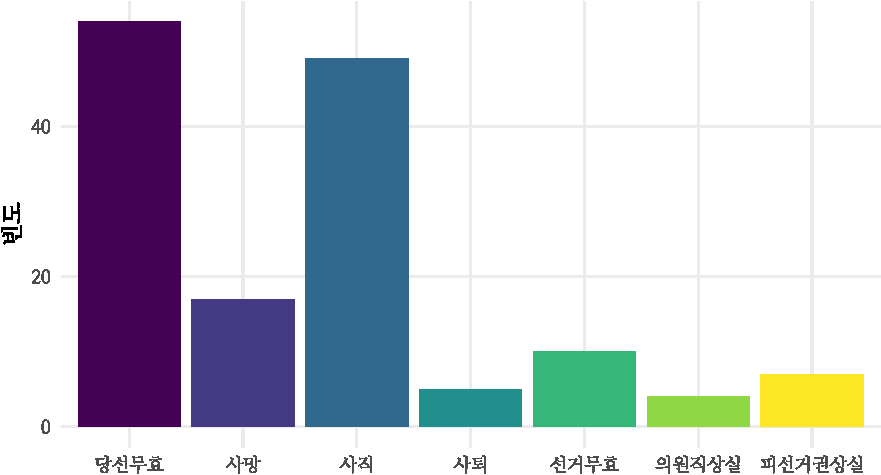
\includegraphics{Codebook_national_files/figure-latex/unnamed-chunk-3-1.pdf}
\caption{재보궐 선거 사유}
\end{figure}

\begin{description}
\item[ELEC\_REASON\_RE]
재보궐 시행 사유 (재코딩, FCT). 1: 일신상의 이유로 사직/사퇴, 2: 비위를
저질렀으나 스스로 사직/사퇴, 3: 비위로 인하여 사법적으로
당선무효/선거무효 처리
\end{description}

\begin{table}[H]

\caption{재보궐 선거 시행 사유}
\centering
\begin{tabular}[t]{l|r|r|r}
\hline
  & 일신상의  & 비위로 인한 & 비위로 인해\\
  & 이유로 사직/사퇴 & 자진 사직/사퇴 & 사법적 당선무효/선거무효\\
\hline
당선무효 & 0 & 2 & 52\\
\hline
사망 & 17 & 0 & 0\\
\hline
사직 & 42 & 6 & 1\\
\hline
사퇴 & 0 & 5 & 0\\
\hline
선거무효 & 0 & 0 & 10\\
\hline
의원직상실 & 0 & 0 & 4\\
\hline
피선거권상실 & 0 & 0 & 7\\
\hline
\end{tabular}
\end{table}

\begin{figure}
\centering
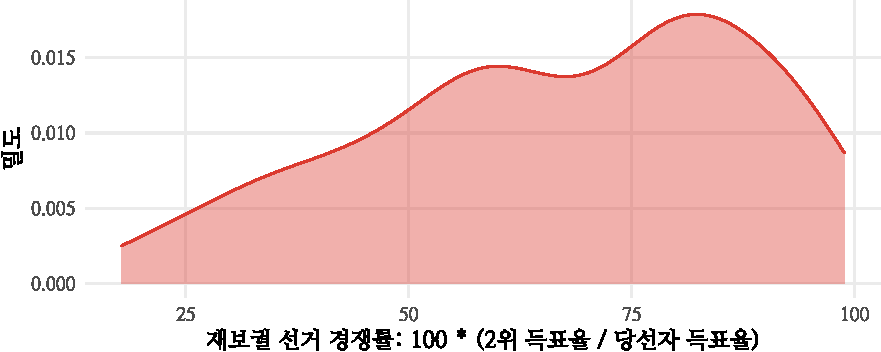
\includegraphics{Codebook_national_files/figure-latex/unnamed-chunk-5-1.pdf}
\caption{재보궐 시행 사유별 투표율}
\end{figure}

\begin{description}
\item[ELEC\_COMPETE]
재보궐경쟁률(NUM), 100 * (2위 득표자 득표율 / 해당 재보궐 선거에서
당선자 득표율).
\end{description}

\begin{figure}
\centering
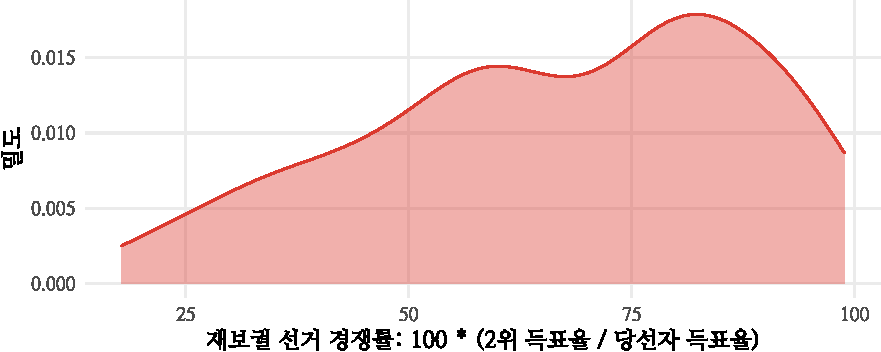
\includegraphics{Codebook_national_files/figure-latex/unnamed-chunk-6-1.pdf}
\caption{재보궐 선거 경쟁률의 분포}
\end{figure}

\begin{figure}
\centering
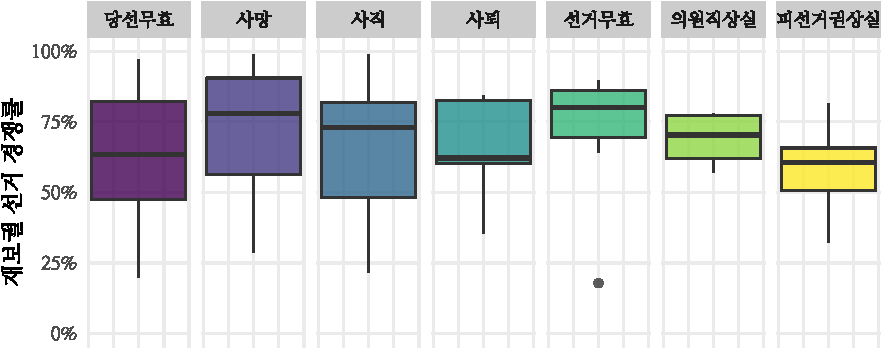
\includegraphics{Codebook_national_files/figure-latex/unnamed-chunk-7-1.pdf}
\caption{재보궐 시행 사유별 경쟁률}
\end{figure}

\begin{description}
\item[ELEC\_COMPETE1]
재보궐경쟁률(NUM), 1위 당선자 득표율 - 2위 후보자 득표율 (윤종빈 2006;
엄기홍 2012).
\end{description}

\begin{figure}
\centering
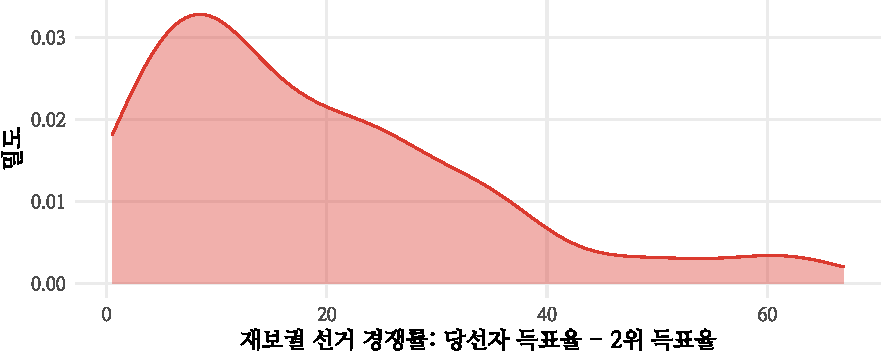
\includegraphics{Codebook_national_files/figure-latex/unnamed-chunk-8-1.pdf}
\caption{재보궐 선거 경쟁률의 분포}
\end{figure}

\begin{description}
\item[ELEC\_COMPETE2]
재보궐경쟁률(NUM), (1위 당선자 득표율 - 2위 후보 득표율)/(1위 당선자
득표율 + 2위 후보 득표율) (김지윤 2010).
\end{description}

\begin{figure}
\centering
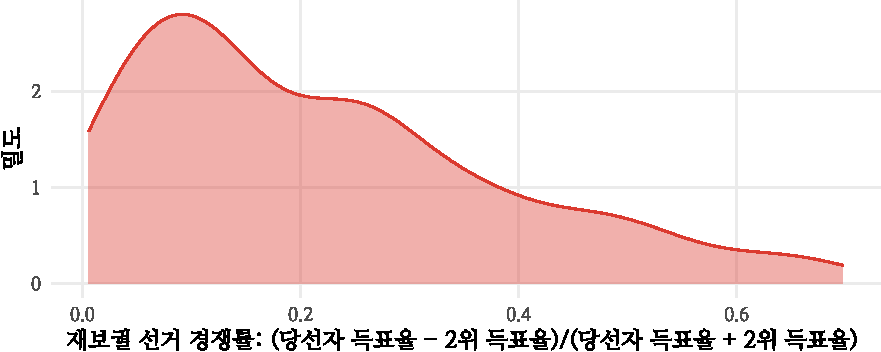
\includegraphics{Codebook_national_files/figure-latex/unnamed-chunk-9-1.pdf}
\caption{재보궐 선거 경쟁률의 분포}
\end{figure}

\begin{description}
\item[ELEC\_COMPETE3]
재보궐경쟁률(NUM), 1 - ((1위 당선자 득표수 - 2위 후보자 득표수)/(1위
당선자 득표수 + 2위 후보자 득표수)) (황아란 2011).
\end{description}

\begin{figure}
\centering
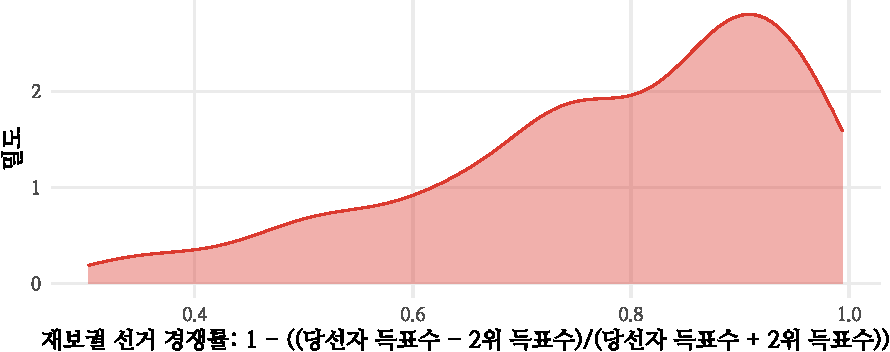
\includegraphics{Codebook_national_files/figure-latex/unnamed-chunk-10-1.pdf}
\caption{재보궐 선거 경쟁률의 분포}
\end{figure}

\begin{longtable}[t]{l|r|r|r|r}
\caption{\label{tab:unnamed-chunk-11}재보궐경쟁률 측정지표의 상관관계표}\\
\hline
  & 선거경쟁도 & 선거경쟁도1 & 선거경쟁도2 & 선거경쟁도3\\
\hline
선거경쟁도 & 1.00 & -0.96 & -0.99 & 0.99\\
\hline
선거경쟁도1 & -0.96 & 1.00 & 0.98 & -0.98\\
\hline
선거경쟁도2 & -0.99 & 0.98 & 1.00 & -1.00\\
\hline
선거경쟁도3 & 0.99 & -0.98 & -1.00 & 1.00\\
\hline
\end{longtable}

\begin{description}
\item[ELEC\_CANDINUM]
재보궐후보자수(NUM), 해당 재보궐 선거에 참여한 후보의 수.
\item[ELEC\_EFFECTNUM]
재보궐 유효후보자수(NUM), 해당 재보궐 선거에 참여한 득표율 3\% 이상의
유효후보의 수.
\end{description}

\newpage

\hypertarget{uxc7acuxbcf4uxad90-uxb2f9uxc120uxc790-uxbcc0uxc218}{%
\subsection{재보궐 당선자
변수}\label{uxc7acuxbcf4uxad90-uxb2f9uxc120uxc790-uxbcc0uxc218}}

\begin{description}
\item[ELEC\_PARTY]
당선자당적(CHR) 재보궐선거 당선자의 당적.
\item[ELEC\_ELECTED]
당선자명(CHR), 재보궐선거 당선자의 이름.
\item[ELEC\_GENDER]
당선자 성별(CHR), 재보궐선거 당선자의 성별 (남/여).
\item[ELEC\_SHARE]
당선자득표율(NUM), 재보궐 선거 당선자의 득표율.
\item[ELEC\_NUMBER]
선수(NUM), 재보궐 선거 당선자의 당선 당시 선수 (초선/재선/3선 등).
\end{description}

\hypertarget{uxc7acuxbcf4uxad90-2uxc704uxb4dduxd45cuxc790-uxbcc0uxc218}{%
\subsection{재보궐 2위득표자
변수}\label{uxc7acuxbcf4uxad90-2uxc704uxb4dduxd45cuxc790-uxbcc0uxc218}}

\begin{description}
\item[RIVAL\_PARTY]
2위득표자당적(CHR), 재보궐 선거 2위 득표자의 당적.
\item[RIVAL\_NAME]
2위득표자명(CHR), 재보궐 선거 2위 득표자의 이름.
\item[RIVAL\_GENDER]
2위득표자성별(CHR), 재보궐선거 2위 득표자의 성별 (남/여).
\item[RIVAL\_SHARE]
2위득표자득표율(NUM), 재보궐 선거 2위 득표자의 득표율.
\end{description}

\hypertarget{uxc7acuxbcf4uxad90-uxc120uxac70-uxc9c1uxc804-uxcd1duxc120-uxbcc0uxc218}{%
\subsection{재보궐 선거 직전 총선
변수}\label{uxc7acuxbcf4uxad90-uxc120uxac70-uxc9c1uxc804-uxcd1duxc120-uxbcc0uxc218}}

\begin{description}
\item[PRE\_POP]
직전총선선거인수(NUM), 해당 재보궐 선거 직전의 총선을 대상으로
선거통계시스템에서 인용한 총 선거인 수.
\item[PRE\_VOTER]
직전총선투표인수(NUM), 해당 재보궐 선거 직전의 총선을 대상으로
선거통계시스템에서 인용한 총 투표인 수.
\item[PRE\_RESIGN]
직전총선기권자수(NUM), 해당 재보궐 선거 직전의 총선을 대상으로 계산한
기권자 수: 선거인 수 - 총 투표인 수.
\item[PRE\_TURNOUT]
직전총선투표율(NUM), 해당 재보궐 선거 직전의 총선을 대상으로 계산한
투표율: 총 투표인 수 / 총 유권자 수 * 100, 소수점 둘째자리로 반올림.
\end{description}

\begin{figure}
\centering
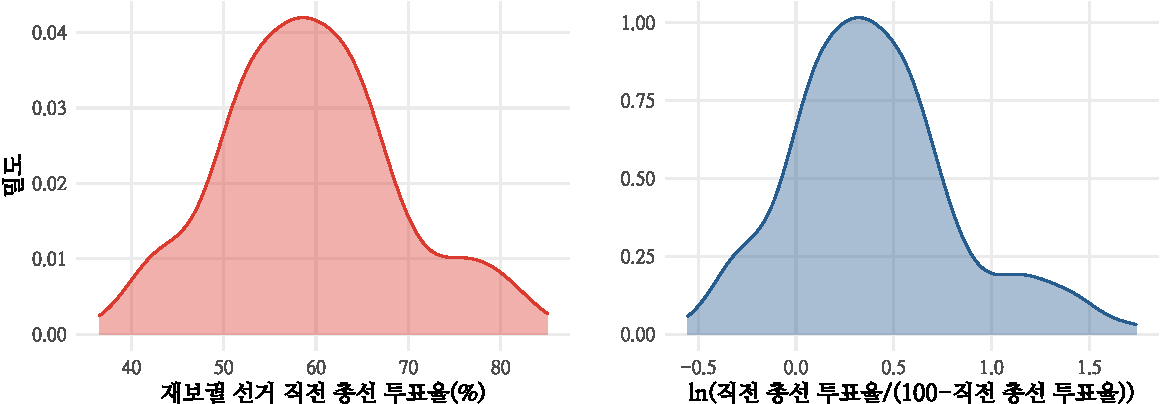
\includegraphics{Codebook_national_files/figure-latex/unnamed-chunk-13-1.pdf}
\caption{재보궐 선거 직전 총선 투표율 변수의 분포}
\end{figure}

\begin{description}
\item[PRE\_PARTY]
직전당선자당적(CHR), 해당 재보궐 선거 직전에 당선자의 당적.
\item[PRE\_ELECTED]
직전당선자(CHR), 해당 재보궐 선거 직전에 당선된 자의 이름.
\item[PRE\_SHARE]
직전총선당선득표율(NUM), 해당 재보궐 선거 직전의 총선에서 당선자의
득표율.
\item[PRE\_RIVAL\_SHARE]
직전총선2위득표율(NUM), 해당 재보궐 선거 직전의 총선에서 2위 득표자의
득표율.
\item[PRE\_COMPETE]
직전선거경쟁률(NUM), 100 * (2위 득표자 득표율 / 해당 재보궐 선거 직전의
총선에서 당선자 득표율).
\end{description}

\begin{figure}
\centering
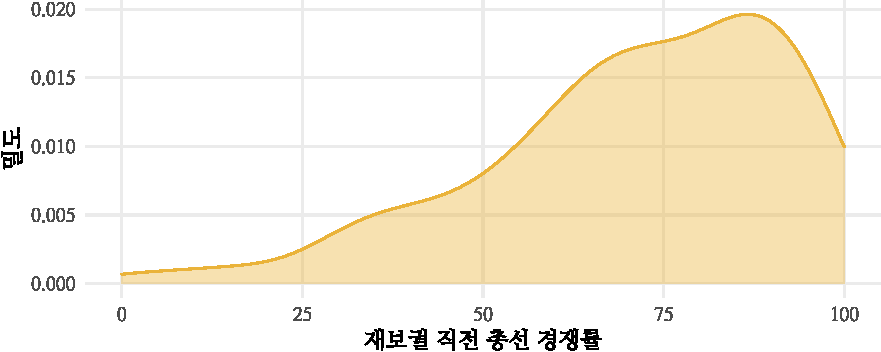
\includegraphics{Codebook_national_files/figure-latex/unnamed-chunk-14-1.pdf}
\caption{재보궐 직전 총선 경쟁률의 분포}
\end{figure}

\begin{description}
\item[PRE\_CANDINUM]
직전선거후보자수(NUM), 해당 재보궐 선거 직전의 총선에 참여한 후보의 수.
\item[PRE\_EFFECTNUM]
직전선거 유효후보자수(NUM), 해당 재보궐 선거 직전의 총선에 참여한 득표율
3\% 이상의 유효후보의 수.
\end{description}

\begin{figure}
\centering
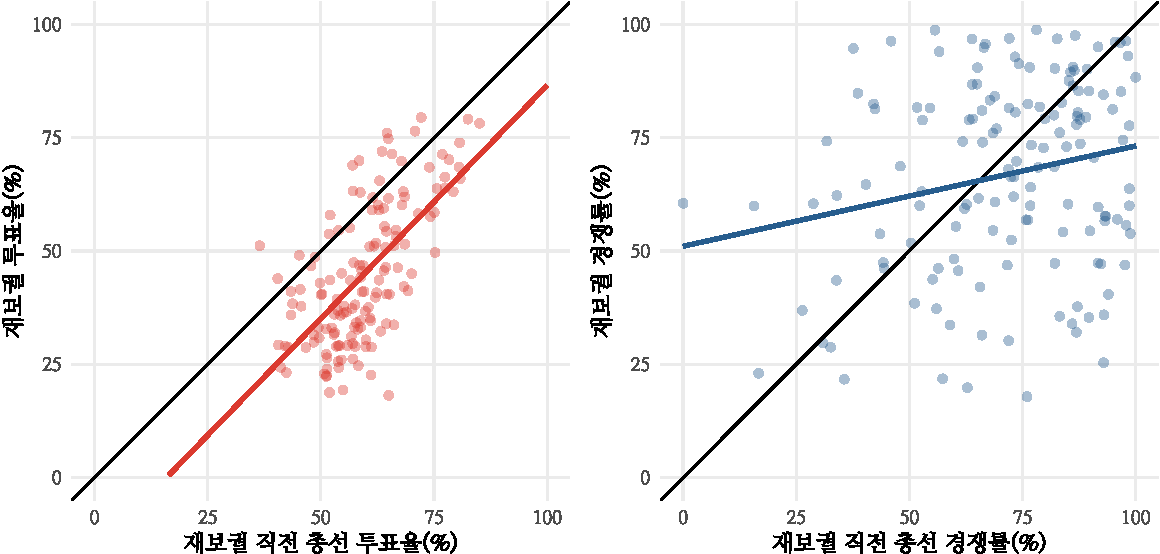
\includegraphics{Codebook_national_files/figure-latex/unnamed-chunk-15-1.pdf}
\caption{재보궐 선거 직전 총선 투표율과 재보궐 선거 투표율 간 관계}
\end{figure}

\newpage

\hypertarget{uxc7acuxbcf4uxad90-uxc120uxac70-uxc9c1uxd6c4-uxcd1duxc120-uxbcc0uxc218}{%
\subsection{재보궐 선거 직후 총선
변수}\label{uxc7acuxbcf4uxad90-uxc120uxac70-uxc9c1uxd6c4-uxcd1duxc120-uxbcc0uxc218}}

\begin{description}
\item[POST\_POP]
직후총선선거인수(NUM), 해당 재보궐 선거 직후의 총선을 대상으로
선거통계시스템에서 인용한 총 선거인 수.
\item[POST\_VOTER]
직후총선투표인수(NUM), 해당 재보궐 선거 직후의 총선을 대상으로
선거통계시스템에서 인용한 총 투표인 수.
\item[POST\_RESIGN]
직후총선기권자수(NUM), 해당 재보궐 선거 직후의 총선을 대상으로 계산한
기권자 수: 선거인 수 - 총 투표인 수.
\item[POST\_TURNOUT]
직후총선투표율(NUM), 해당 재보궐 선거 직후의 총선을 대상으로 계산한
투표율: 총 투표인 수 / 총 유권자 수 * 100, 소수점 둘째자리로 반올림.
\end{description}

\begin{figure}
\centering
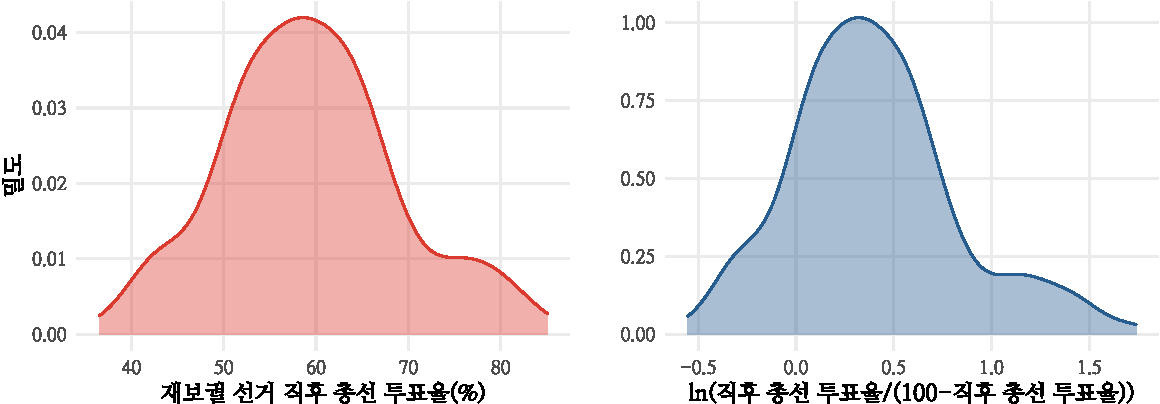
\includegraphics{Codebook_national_files/figure-latex/unnamed-chunk-16-1.pdf}
\caption{재보궐 선거 직후 총선 투표율 변수의 분포}
\end{figure}

\begin{description}
\item[POST\_PARTY]
직후당선자당적(CHR), 해당 재보궐 선거 직후의 총선에서 당선자의 당적.
\item[POST\_ELECTED]
직후당선자(CHR), 해당 재보궐 선거 직후의 총선에서 당선자의 이름.
\item[POST\_SHARE]
직후총선당선득표율(NUM), 해당 재보궐 선거 직후의 총선에서 당선자의
득표율.
\item[POST\_RIVAL\_SHARE]
직후총선2위득표율(NUM), 해당 재보궐 선거 직후의 총선에서 2위 득표자의
득표율.
\item[POST\_COMPETE]
직후총선경쟁률(NUM), 100 * (2위 득표자 득표율 / 해당 재보궐 선거 직후의
총선에서 당선자 득표율).
\end{description}

\begin{figure}
\centering
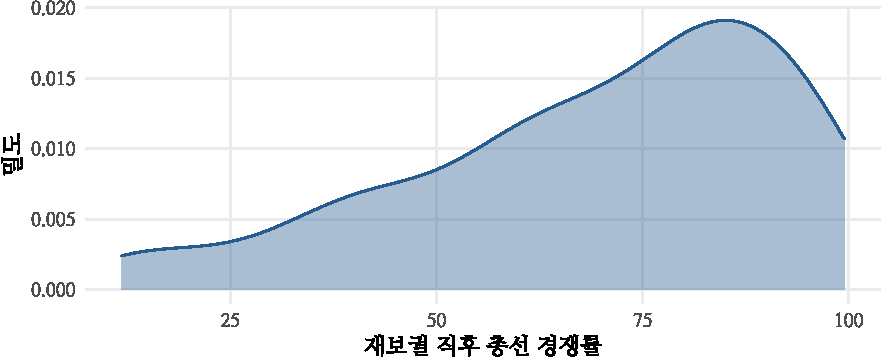
\includegraphics{Codebook_national_files/figure-latex/unnamed-chunk-17-1.pdf}
\caption{재보궐 직후 총선 경쟁률의 분포}
\end{figure}

\begin{description}
\item[POST\_CANDINUM]
직후선거후보자수(NUM), 해당 재보궐 선거 직후의 총선에 참여한 후보의 수.
\item[POST\_EFFECTNUM]
직후선거 유효후보자수(NUM), 해당 재보궐 선거 직후의 총선에 참여한 득표율
3\% 이상의 유효후보의 수.
\end{description}

\hypertarget{uxae30uxd0c0-uxc120uxac70-uxad00uxb828-uxbcc0uxc218}{%
\subsection{기타 선거 관련
변수}\label{uxae30uxd0c0-uxc120uxac70-uxad00uxb828-uxbcc0uxc218}}

\begin{description}
\item[GENERAL\_DATE]
인접총선일자(DATE), 재보궐 선거로부터 가장 가까운 미래 인접 총선의 일자.
\item[GENERAL\_DIFF]
인접총선일자차이(NUM), 인접총선일자 - 선거일.
\item[GENERAL\_TENURE]
의회임기\_남은햇수(NUM), 재보궐 선거 당시 남은 의회 임기(햇수).
\item[PRESIDENT]
역대 대통령
\end{description}

\begin{figure}
\centering
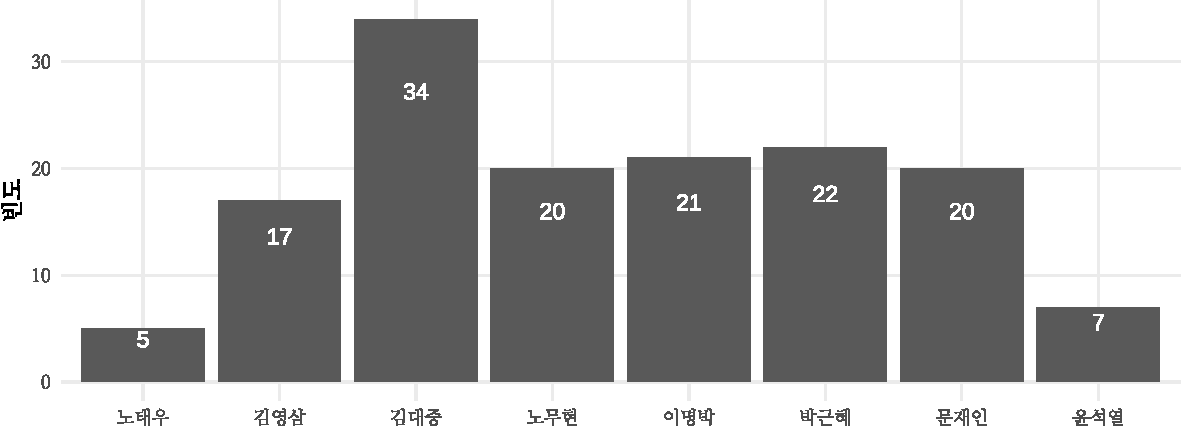
\includegraphics{Codebook_national_files/figure-latex/unnamed-chunk-18-1.pdf}
\caption{역대 대통령 임기 중 재보궐 선거 수}
\end{figure}

\begin{description}
\item[PRESIDENT\_DATE]
인접 대선 일자(DATE), 재보궐 선거로부터 가장 가까운 미래 인접 대선의
일자.
\item[PRESIDENT\_DIFF]
인접 대선 일자 차이(NUM), 인접대선일자 - 선거일.
\item[PRESIDENT\_TENURE]
대통령임기\_남은햇수(NUM), 재보궐 선거 당시 남은 대통령 임기(햇수).
\item[LOCAL\_DATE]
인접 지선 일자(DATE), 재보궐 선거로부터 가장 가까운 미래 인접 지선의
일자.
\item[LOCAL\_DIFF]
인접 지선 일자 차이(NUM), 인접지선일자 - 선거일.
\item[NATL\_DATE]
인접 전국단위 선거일자(DATE), 재보궐 선거로부터 가장 가까운 미래 인접
전국단위 선거의 일자.
\item[NATL\_DIFF]
인접 전국단위 선거 일자 차이(NUM), 인접 전국단위 선거 일자 - 선거일.
\end{description}

\begin{figure}
\centering
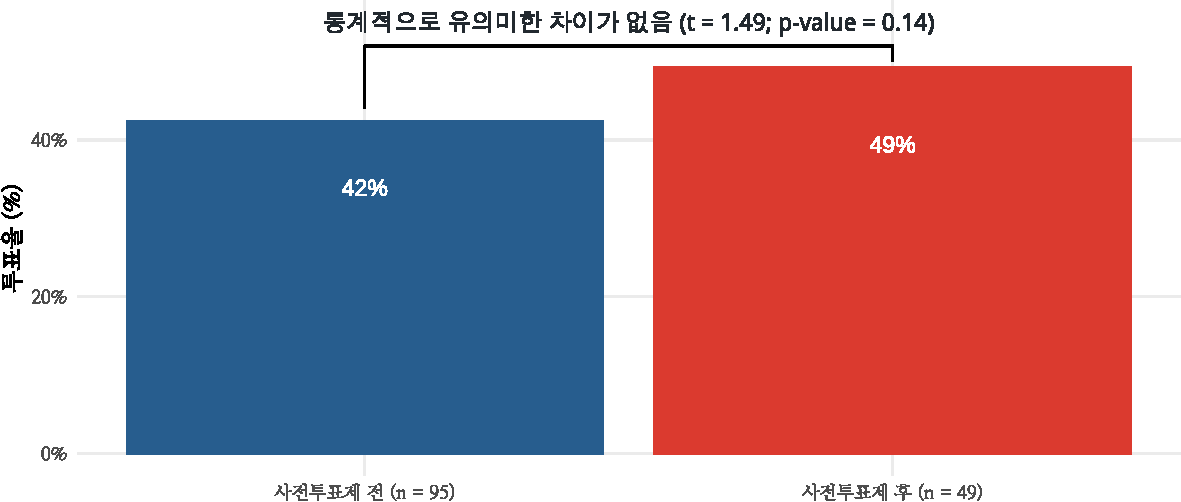
\includegraphics{Codebook_national_files/figure-latex/unnamed-chunk-19-1.pdf}
\caption{재보궐 선거와 인접 선거 간 일자 차이 (총선/대선/지선/전국단위
선거)}
\end{figure}

\newpage

\begin{description}
\item[PRESIDENT\_POSITIVE]
대통령\_평가(긍정)(NUM), 재보궐선거가 실시된 시점 이전의 시기에서 가장
근접한 시점에 조사된 여론조사 전문기관인 한국갤럽이 조사한 주차별 대통령
국정운영 지지율(긍정).
\item[PRESIDENT\_NEGATIVE]
대통령\_평가(부정)(NUM), 재보궐선거가 실시된 시점 이전의 시기에서 가장
근접한 시점에 조사된 여론조사 전문기관인 한국갤럽이 조사한 주차별 대통령
국정운영 지지율(부정).
\end{description}

\begin{figure}
\centering
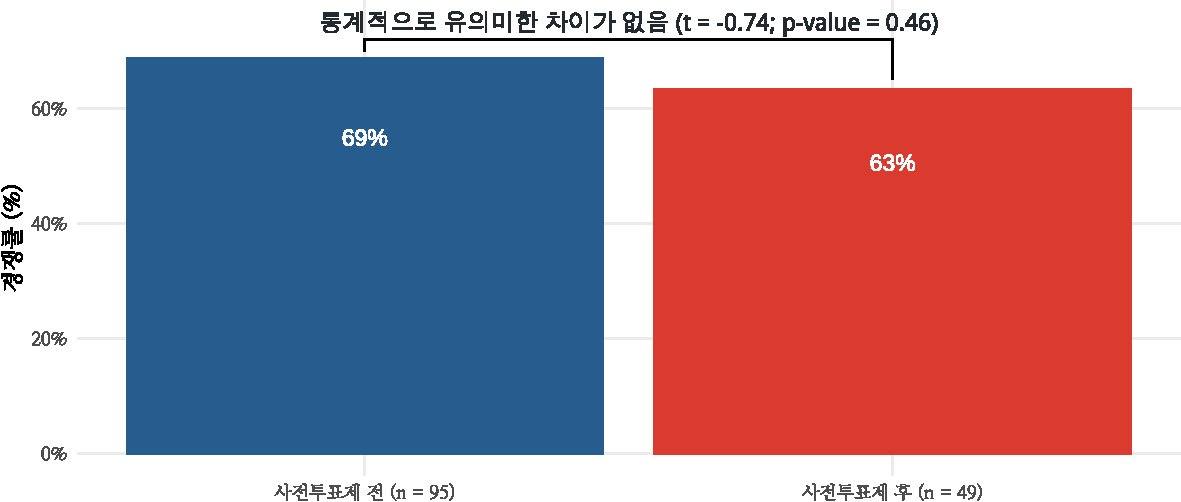
\includegraphics{Codebook_national_files/figure-latex/unnamed-chunk-20-1.pdf}
\caption{대통령 평가 (긍정/부정)}
\end{figure}

\begin{description}
\item[REGIONALISM]
지역주의(FCT), 재보궐 선거가 실시된 지역을 기준으로 지역주의 코딩 (1 =
PK (부울경) / 2 = TK (대구경북) / 3 = HN (호남) / 4 = 기타).
\item[RULINGPARTY]
여당(CHR), 재보궐 선거가 실시된 시점의 여당이름.
\item[RULINGAPPROVAL]
여당지지도(NUM), 재보궐 선거가 실시된 시점 이전의 시기에서 가장 근접한
시점에 조사된 여론조사 전문기관인 리서치앤리서치(R\&R)가 조사한
여당지지율.
\item[PRE\_ELEC\_CANDI\_DIFF]
직전재보궐후보자수차이(NUM), 재보궐 선거에 참여한 후보자 수 - 해당
재보궐 선거 직전의 총선에 참여한 후보의 수.
\item[POST\_ELEC\_CANDI\_DIFF]
직후재보궐후보자수차이(NUM), 해당 재보궐 선거 직후의 총선에 참여한
후보의 수 - 재보궐 선거에 참여한 후보자 수.
\item[PRE\_ELEC\_SHIFT]
재보궐전교체(NUM), 재보궐 이전 총선의 당선자로부터 재보궐 선거 당선자의
당적이 교체된 경우 (이항변수; 1, 0).
\item[POST\_ELEC\_SHIFT]
재보궐이후교체(NUM), 재보궐 선거 당선자로부터 재보궐 이전 총선의
당선자의 당적이 교체된 경우 (이항변수; 1, 0).
\item[PRE\_ELEC\_COMPETE\_DIFF]
직전보궐경쟁률차이(NUM), 재보궐경쟁률 - 직전선거경쟁률.
\item[POST\_ELEC\_COMPETE\_DIFF]
직후보궐경쟁률차이(NUM), 직후선거경쟁률 - 재보궐경쟁률.
\item[PRE\_ELEC\_SHIFT2]
의석교체(FCT), 여당, 직전당선자당적과 당선자당적 변수를 바탕으로 1 =
여당 \(\rightarrow\) 여당 / 2 = 여당 \(\rightarrow\) 야당 / 3 = 야당
\(\rightarrow\) 여당 / 4 = 야당 \(\rightarrow\) 야당.
\item[ELEC\_RULING]
여당유리지역주의(FCT), 선거 당시 여당을 지지하는 지역주의에 선거구가
위치하고 있으면 1 아니면 0.
\item[ELEC\_OPPOSITION]
야당유리지역주의(FCT), 선거 당시 야당을 지지하는 지역주의에 선거구가
위치하고 있으면 1 아니면 0.
\item[PREVOTE]
사전투표제 도입 여부(NUM), 사전투표제도가 도입된 2013년도 상반기
재·보궐선거 이후 선거일 경우 1, 아니면 0.
\end{description}

\begin{figure}
\centering
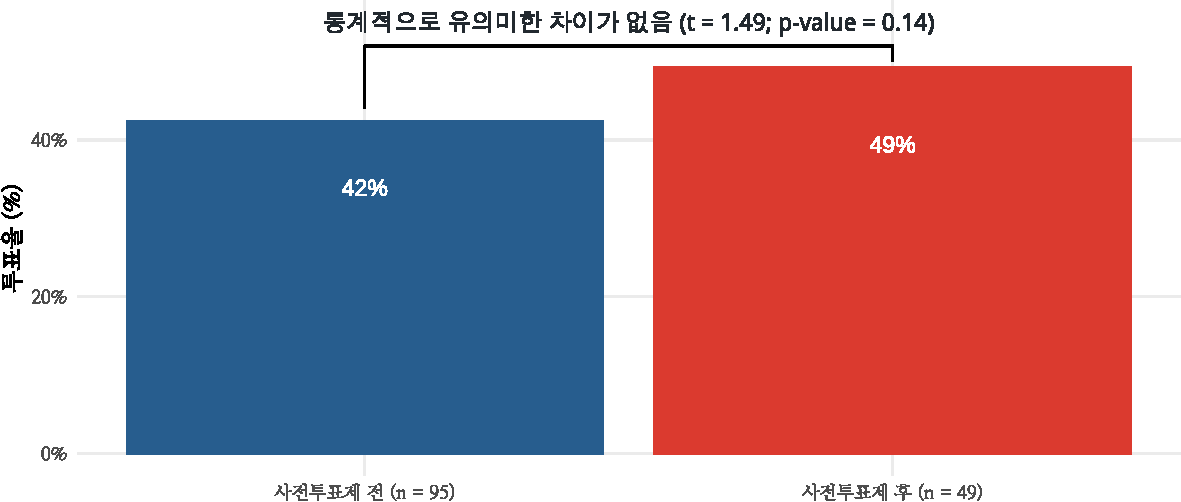
\includegraphics{Codebook_national_files/figure-latex/unnamed-chunk-21-1.pdf}
\caption{사전투표제도 도입 전후 재보궐선거 투표율 비교(평균)}
\end{figure}

\begin{figure}
\centering
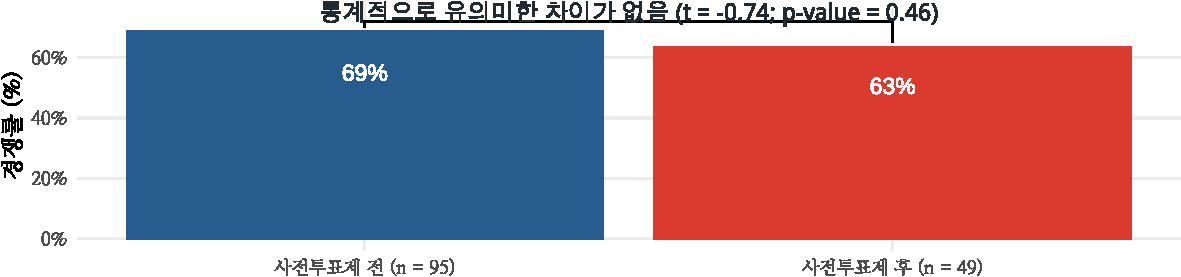
\includegraphics{Codebook_national_files/figure-latex/unnamed-chunk-22-1.pdf}
\caption{사전투표제도 도입 전후 재보궐선거 경쟁률 비교(평균)}
\end{figure}

\begin{description}
\item[METROPOL]
지역구 도시 규모(FCT), 광역시 및 특별시 = 1 / 중소도시 = 2 / 읍면지역 =
3.
\end{description}

\begin{figure}
\centering
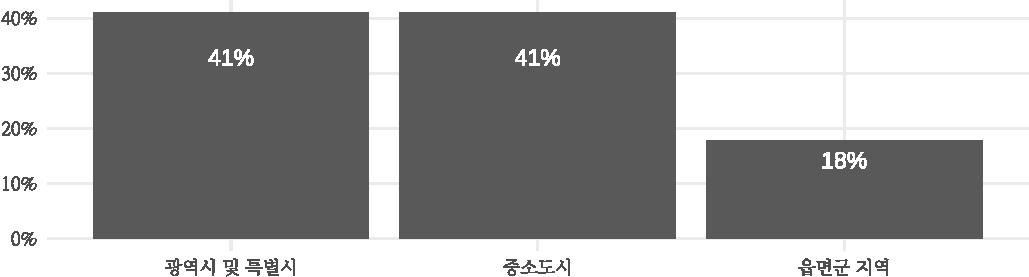
\includegraphics{Codebook_national_files/figure-latex/unnamed-chunk-23-1.pdf}
\caption{재보궐 선거 시행 선거구의 도시 규모}
\end{figure}

\newpage

\hypertarget{appendix}{%
\section{APPENDIX}\label{appendix}}

\hypertarget{uxc7acuxbcf4uxad90-uxc120uxac70-uxc9c0uxc5eduxad6cuxc5d0-uxb300uxd55c-uxac04uxb7b5uxd55c-uxc815uxbcf4}{%
\subsection{재보궐 선거 지역구에 대한 간략한
정보}\label{uxc7acuxbcf4uxad90-uxc120uxac70-uxc9c0uxc5eduxad6cuxc5d0-uxb300uxd55c-uxac04uxb7b5uxd55c-uxc815uxbcf4}}

\begin{longtable}[t]{l|l|l|l|r}
\caption{\label{tab:unnamed-chunk-24}재보궐선거 지역구 및 재보궐 사유에 대한 정보}\\
\hline
재보궐 선거일 & 시도 & 지역구 & 재보궐 사유 & 투표율\\
\hline
1989-04-14 & 강원도 & 동해시 & 당선무효 & 79.1\\
\hline
1989-08-18 & 서울시 & 영등포을 & 당선무효 & 69.8\\
\hline
1990-04-03 & 대구시 & 서구갑 & 사퇴 & 63.9\\
\hline
1990-04-03 & 충청북도 & 진천음성군 & 사망 & 78.2\\
\hline
1990-11-09 & 전라남도 & 영광함평군 & 당선무효 & 70.2\\
\hline
1993-04-23 & 부산시 & 동래구갑 & 사직 & 40.4\\
\hline
1993-04-23 & 부산시 & 사하구 & 당선무효 & 42.1\\
\hline
1993-04-23 & 경기도 & 광명시 & 사망 & 41.2\\
\hline
1993-06-11 & 강원도 & 명주양양군 & 사퇴 & 68.5\\
\hline
1993-06-11 & 강원도 & 철원화천군 & 사퇴 & 66.0\\
\hline
1993-06-11 & 경상북도 & 예천군 & 사퇴 & 71.3\\
\hline
1993-08-12 & 대구시 & 동구을 & 사퇴 & 60.2\\
\hline
1993-08-12 & 강원도 & 춘천시 & 사망 & 58.5\\
\hline
1994-08-02 & 대구시 & 수성갑 & 당선무효 & 46.3\\
\hline
1994-08-02 & 강원도 & 영월평창군 & 사망 & 63.1\\
\hline
1994-08-02 & 경상북도 & 경주시 & 사망 & 49.7\\
\hline
1997-03-05 & 인천시 & 서구 & 사망 & 37.3\\
\hline
1997-03-05 & 경기도 & 수원시장안구 & 사망 & 32.7\\
\hline
1997-07-24 & 경상북도 & 포항시북구 & 당선무효 & 63.1\\
\hline
1997-07-24 & 충청남도 & 예산군 & 당선무효 & 68.5\\
\hline
1997-09-04 & 경기도 & 안양시만안구 & 사망 & 33.1\\
\hline
1997-12-28 & 광주시 & 동구 & 사망 & NA\\
\hline
1998-04-02 & 부산시 & 서구 & 당선무효 & 45.7\\
\hline
1998-04-02 & 대구시 & 달성군 & 사직 & 59.4\\
\hline
1998-04-02 & 경상북도 & 문경시예천군 & 당선무효 & 66.3\\
\hline
1998-04-02 & 경상북도 & 의성군 & 당선무효 & 73.9\\
\hline
1998-07-21 & 서울시 & 종로구 & 사직 & 33.7\\
\hline
1998-07-21 & 서울시 & 서초구갑 & 사직 & 37.6\\
\hline
1998-07-21 & 부산시 & 해운대구기장군을 & 사직 & 58.3\\
\hline
1998-07-21 & 대구시 & 북구갑 & 사직 & 39.8\\
\hline
1998-07-21 & 경기도 & 수원시팔달구 & 사망 & 26.2\\
\hline
1998-07-21 & 경기도 & 광명시을 & 사직 & 50.8\\
\hline
1998-07-21 & 강원도 & 강릉시을 & 당선무효 & 54.6\\
\hline
1999-03-30 & 서울시 & 구로구을 & 당선무효 & 40.8\\
\hline
1999-03-30 & 경기도 & 시흥시 & 사망 & 32.2\\
\hline
1999-06-03 & 서울시 & 송파구갑 & 당선무효 & 46.4\\
\hline
1999-06-03 & 인천시 & 계양구강화군갑 & 당선무효 & 35.2\\
\hline
2001-10-25 & 서울시 & 동대문구을 & 선거무효 & 45.6\\
\hline
2001-10-25 & 서울시 & 구로구을 & 당선무효 & 39.4\\
\hline
2001-10-25 & 강원도 & 강릉시 & 사직 & 41.0\\
\hline
2002-08-08 & 서울시 & 종로구 & 당선무효 & 28.9\\
\hline
2002-08-08 & 서울시 & 금천구 & 당선무효 & 24.3\\
\hline
2002-08-08 & 서울시 & 영등포을 & 사직 & 24.0\\
\hline
2002-08-08 & 부산시 & 부산진갑 & 당선무효 & 29.1\\
\hline
2002-08-08 & 부산시 & 해운대기장갑 & 사망 & 18.8\\
\hline
2002-08-08 & 인천시 & 서구 강화군을 & 당선무효 & 34.0\\
\hline
2002-08-08 & 광주시 & 광주 북구갑 & 사직 & 22.4\\
\hline
2002-08-08 & 경기도 & 광명시 & 사직 & 30.4\\
\hline
2002-08-08 & 경기도 & 하남시 & 당선무효 & 36.3\\
\hline
2002-08-08 & 경기도 & 안성시 & 사망 & 43.5\\
\hline
2002-08-08 & 전라북도 & 군산시 & 사직 & 33.2\\
\hline
2002-08-08 & 경상남도 & 마산합포구 & 당선무효 & 29.6\\
\hline
2002-08-08 & 제주시 & 북제주군 & 당선무효 & 57.6\\
\hline
2002-12-19 & 울산시 & 중구 & 사망 & 68.9\\
\hline
2003-04-24 & 서울시 & 양천구을 & 사직 & 26.4\\
\hline
2003-04-24 & 경기도 & 의정부시 & 사직 & 26.0\\
\hline
2003-04-24 & 경기도 & 고양시덕양구갑 & 당선무효 & 25.6\\
\hline
2005-04-30 & 경기도 & 성남시중원구 & 당선무효 & 29.1\\
\hline
2005-04-30 & 경기도 & 포천시연천군 & 당선무효 & 38.1\\
\hline
2005-04-30 & 충청남도 & 공주시연기군 & 당선무효 & 37.9\\
\hline
2005-04-30 & 충청남도 & 아산시 & 당선무효 & 32.0\\
\hline
2005-04-30 & 경상북도 & 영천시 & 당선무효 & 59.1\\
\hline
2005-04-30 & 경상남도 & 김해시갑 & 당선무효 & 34.2\\
\hline
2005-10-26 & 대구시 & 동구을 & 당선무효 & 46.9\\
\hline
2005-10-26 & 울산시 & 북구 & 당선무효 & 53.2\\
\hline
2005-10-26 & 경기도 & 부천시원미구갑 & 당선무효 & 28.9\\
\hline
2005-10-26 & 경기도 & 광주시 & 당선무효 & 36.7\\
\hline
2006-07-26 & 서울시 & 성북구을 & 당선무효 & 28.9\\
\hline
2006-07-26 & 서울시 & 송파구갑 & 사직 & 18.1\\
\hline
2006-07-26 & 경기도 & 부천시소사구 & 사직 & 22.6\\
\hline
2006-07-26 & 경상남도 & 마산시갑 & 당선무효 & 28.8\\
\hline
2006-10-25 & 인천시 & 남동구을 & 피선거권상실 & 24.7\\
\hline
2006-10-25 & 전라남도 & 해남진도 & 피선거권상실 & 40.5\\
\hline
2007-04-25 & 대전시 & 서구을 & 사망 & 34.6\\
\hline
2007-04-25 & 경기도 & 화성시 & 피선거권상실 & 19.3\\
\hline
2007-04-25 & 전라남도 & 무안신안 & 피선거권상실 & 54.4\\
\hline
2009-04-29 & 인천시 & 부평구을 & 선거무효 & 29.1\\
\hline
2009-04-29 & 울산시 & 북구 & 선거무효 & 46.7\\
\hline
2009-04-29 & 전라북도 & 전주시완산구갑 & 선거무효 & 37.8\\
\hline
2009-04-29 & 전라북도 & 전주시덕진구 & 선거무효 & 38.4\\
\hline
2009-04-29 & 경상북도 & 경주시 & 선거무효 & 53.8\\
\hline
2009-10-28 & 경기도 & 수원시장안구 & 선거무효 & 35.8\\
\hline
2009-10-28 & 경기도 & 안산시상록구을 & 선거무효 & 29.3\\
\hline
2009-10-28 & 강원도 & 강릉시 & 선거무효 & 40.3\\
\hline
2009-10-28 & 충청북도 & 증평진천괴산음성군 & 피선거권상실 & 42.9\\
\hline
2009-10-28 & 경상남도 & 양산시 & 선거무효 & 43.9\\
\hline
2010-07-28 & 서울시 & 은평구을 & 당선무효 & 40.5\\
\hline
2010-07-28 & 인천시 & 계양구을 & 사직 & 23.2\\
\hline
2010-07-28 & 광주시 & 남구 & 사직 & 28.7\\
\hline
2010-07-28 & 강원도 & 원주시 & 사직 & 28.7\\
\hline
2010-07-28 & 강원도 & 태백시영월군평창군정선군 & 사직 & 45.1\\
\hline
2010-07-28 & 강원도 & 철원군화천군양구군인제군 & 사망 & 47.4\\
\hline
2010-07-28 & 충청북도 & 충주시 & 사직 & 43.6\\
\hline
2010-07-28 & 충청남도 & 천안시을 & 사직 & 24.3\\
\hline
2011-04-27 & 경기도 & 성남시분당구을 & 사직 & 49.1\\
\hline
2011-04-27 & 전라남도 & 순천시 & 당선무효 & 41.1\\
\hline
2011-04-27 & 경상남도 & 김해시을 & 당선무효 & 41.5\\
\hline
2013-04-24 & 서울시 & 노원구병 & 의원직상실 & 43.5\\
\hline
2013-04-24 & 부산시 & 영도구 & 당선무효 & 36.0\\
\hline
2013-04-24 & 충청남도 & 부여군청양군 & 당선무효 & 44.2\\
\hline
2014-07-30 & 서울시 & 동작구을 & 사직 & 46.8\\
\hline
2014-07-30 & 부산시 & 해운대구기장군갑 & 사직 & 22.9\\
\hline
2014-07-30 & 광주시 & 광산구을 & 사직 & 22.3\\
\hline
2014-07-30 & 대전시 & 대덕구 & 사직 & 32.7\\
\hline
2014-07-30 & 울산시 & 남구을 & 사직 & 29.1\\
\hline
2014-07-30 & 경기도 & 평택시을 & 당선무효 & 29.8\\
\hline
2014-07-30 & 경기도 & 수원시을 & 당선무효 & 27.2\\
\hline
2014-07-30 & 경기도 & 수원시병 & 사직 & 30.8\\
\hline
2014-07-30 & 경기도 & 수원시정 & 사직 & 31.1\\
\hline
2014-07-30 & 경기도 & 김포시 & 사직 & 35.8\\
\hline
2014-07-30 & 충청남도 & 서산시태안군 & 당선무효 & 33.0\\
\hline
2014-07-30 & 충청북도 & 충주시 & 사직 & 33.1\\
\hline
2014-07-30 & 전라남도 & 담양군함평군영광군장성군 & 사직 & 31.6\\
\hline
2014-07-30 & 전라남도 & 나주시화순군 & 당선무효 & 34.6\\
\hline
2014-07-30 & 전라남도 & 순천시곡성군 & 피선거권상실 & 51.0\\
\hline
2015-04-29 & 서울시 & 관악구을 & 의원직상실 & 36.9\\
\hline
2015-04-29 & 인천시 & 서구강화군을 & 당선무효 & 36.5\\
\hline
2015-04-29 & 광주시 & 서구을 & 의원직상실 & 41.1\\
\hline
2015-04-29 & 경기도 & 성남시중원구 & 의원직상실 & 31.5\\
\hline
2017-04-12 & 경상북도 & 상주시군위군의성군청송군 & 당선무효 & 51.7\\
\hline
2018-06-13 & 서울시 & 노원구병 & 사직 & 61.6\\
\hline
2018-06-13 & 서울시 & 송파구을 & 당선무효 & 62.9\\
\hline
2018-06-13 & 부산시 & 해운대구을 & 사직 & 57.9\\
\hline
2018-06-13 & 인천시 & 남동구갑 & 사직 & 54.5\\
\hline
2018-06-13 & 광주시 & 서구갑 & 당선무효 & 59.1\\
\hline
2018-06-13 & 울산시 & 북구 & 당선무효 & 65.5\\
\hline
2018-06-13 & 충청북도 & 제천시단양군 & 당선무효 & 63.3\\
\hline
2018-06-13 & 충청남도 & 천안시갑 & 당선무효 & 48.6\\
\hline
2018-06-13 & 충청남도 & 천안시병 & 사직 & 55.2\\
\hline
2018-06-13 & 전라남도 & 영암군무안군신안군 & 당선무효 & 71.4\\
\hline
2018-06-13 & 경상북도 & 김천시 & 사직 & 70.0\\
\hline
2018-06-13 & 경상남도 & 김해시을 & 사직 & 61.8\\
\hline
2019-04-03 & 경상남도 & 창원시성산구 & 사망 & 51.2\\
\hline
2019-04-03 & 경상남도 & 통영시고성군 & 피선거권상실 & 51.2\\
\hline
2022-03-09 & 서울시 & 종로구 & 사직 & 76.4\\
\hline
2022-03-09 & 서울시 & 서초구갑 & 사직 & 79.5\\
\hline
2022-03-09 & 대구시 & 중구남구 & 사직 & 76.0\\
\hline
2022-03-09 & 경기도 & 안성시 & 당선무효 & 72.0\\
\hline
2022-03-09 & 충청북도 & 청주시상당구 & 당선무효 & 74.8\\
\hline
2022-06-01 & 대구시 & 수성구을 & 사직 & 45.0\\
\hline
2022-06-01 & 인천시 & 계양을 & 사직 & 60.1\\
\hline
2022-06-01 & 경기도 & 성남시분당구갑 & 사직 & 63.8\\
\hline
2022-06-01 & 강원도 & 원주시갑 & 사직 & 51.1\\
\hline
2022-06-01 & 충청남도 & 보령시서천군 & 사직 & 62.0\\
\hline
2022-06-01 & 경상남도 & 창원시의창구 & 사직 & 51.5\\
\hline
2022-06-01 & 제주시 & 제주을 & 사직 & 55.4\\
\hline
\end{longtable}

\newpage

\hypertarget{uxc8fcuxc694-uxbcc0uxc218uxc758-uxae30uxc220uxd1b5uxacc4}{%
\subsection{주요 변수의
기술통계}\label{uxc8fcuxc694-uxbcc0uxc218uxc758-uxae30uxc220uxd1b5uxacc4}}

\begin{longtable}[t]{l|r|r|r|r|r}
\caption{\label{tab:unnamed-chunk-25}주요 변수의 기술통계}\\
\hline
변수 & 관측치 & 평균 & 표준편차 & 최소값 & 최대값\\
\hline
ELEC\_VOTER & 145 & 66644.61 & 24909.55 & 27215.00 & 148606.00\\
\hline
ELEC\_TURNOUT & 145 & 44.71 & 15.58 & 18.12 & 79.47\\
\hline
ELEC\_SHARE & 145 & 53.20 & 10.05 & 22.39 & 83.46\\
\hline
RIVAL\_SHARE & 145 & 34.11 & 8.96 & 12.90 & 49.68\\
\hline
ELEC\_COMPETE & 145 & 66.86 & 21.16 & 17.84 & 98.82\\
\hline
ELEC\_GENDER* & 146 & 1.06 & 0.24 & 1.00 & 2.00\\
\hline
PRE\_RESIGN & 146 & 63624.24 & 26608.87 & 10012.00 & 128117.00\\
\hline
PRE\_TURNOUT & 146 & 59.37 & 9.68 & 36.52 & 85.06\\
\hline
PRE\_COMPETE & 146 & 70.94 & 21.09 & 0.00 & 99.98\\
\hline
ELEC\_EFFECNUM & 146 & 3.20 & 1.11 & 1.00 & 6.00\\
\hline
PRE\_VOTER & 146 & 87920.03 & 24311.92 & 41017.00 & 157419.00\\
\hline
PRE\_SHARE & 146 & 50.05 & 11.52 & 0.00 & 89.90\\
\hline
PRE\_RIVAL\_SHARE & 146 & 34.07 & 8.32 & 0.00 & 49.34\\
\hline
PRE\_CANDINUM & 146 & 4.47 & 1.80 & 1.00 & 12.00\\
\hline
POST\_VOTER & 107 & 89583.64 & 22888.56 & 41044.00 & 145744.00\\
\hline
POST\_TURNOUT & 107 & 57.41 & 8.61 & 37.71 & 80.58\\
\hline
POST\_SHARE & 107 & 51.91 & 10.52 & 30.27 & 84.43\\
\hline
POST\_RIVAL\_SHARE & 107 & 34.29 & 9.20 & 9.72 & 48.40\\
\hline
POST\_COMPETE & 107 & 69.61 & 22.66 & 11.86 & 99.44\\
\hline
POST\_CANDINUM & 105 & 4.35 & 1.65 & 2.00 & 11.00\\
\hline
ELEC\_RULING & 146 & 0.16 & 0.37 & 0.00 & 1.00\\
\hline
ELEC\_OPPOSITION & 146 & 0.29 & 0.46 & 0.00 & 1.00\\
\hline
\end{longtable}

\end{document}
